% Nylon-6,6 amide synthesis: querying ModelSEED for analogous reactions/enzymes.
% House style: seahorse colortheme, light chrome tinted from `structure`.
\documentclass[aspectratio=169,10pt]{beamer}
\usetheme{default}
\usecolortheme{seahorse}
\usefonttheme{professionalfonts}
\setbeamertemplate{navigation symbols}{}

\usepackage{graphicx}
\usepackage{booktabs}
\usepackage{xcolor}
\usepackage[skins]{tcolorbox}
\usepackage{tikz}
\graphicspath{{../figures/}}

\definecolor{cInk}{HTML}{0B3D5C}
\definecolor{cAccent}{HTML}{0072B2}
\definecolor{cNIS}{HTML}{D55E00}
\definecolor{cGood}{HTML}{1E8449}
\definecolor{cBad}{HTML}{B03A2E}

% Chrome stays LIGHT, tinted from seahorse's `structure` (house rule): a soft
% bar with dark text, not a dark/navy block.
\setbeamercolor{frametitle}{fg=structure!65!black,bg=structure!28!white}
% Paint the title bar explicitly: setting only fg=white without drawing the
% background leaves white-on-white, i.e. an invisible frame title.
\setbeamertemplate{frametitle}{%
  \nointerlineskip%
  \begin{beamercolorbox}[wd=\paperwidth,ht=3.0ex,dp=1.4ex,leftskip=0.35cm,
                         rightskip=0.35cm]{frametitle}%
    \usebeamerfont{frametitle}\insertframetitle%
  \end{beamercolorbox}%
}
\setbeamerfont{frametitle}{size=\large,series=\bfseries}
\setbeamercolor{block title}{bg=structure!20!white,fg=black}
\setbeamercolor{block body}{bg=structure!8!white}
\setbeamertemplate{footline}[frame number]
\setbeamercolor{footline}{fg=structure!50!black}

\newcommand{\good}[1]{{\color{cGood}\textbf{#1}}}
\newcommand{\bad}[1]{{\color{cBad}#1}}
\newcommand{\nis}[1]{{\color{cNIS}\textbf{#1}}}
\newcommand{\takeaway}[1]{\vfill\begin{tcolorbox}[colback=structure!12!white,
  colframe=structure!60!black,boxrule=0.4pt,left=5pt,right=5pt,top=3pt,bottom=3pt]
  \small #1\end{tcolorbox}}

\title{\textbf{Is there an enzyme for nylon-6,6?}}
\subtitle{Querying 33{,}246 ModelSEED reactions with the encoded diad-forming reaction}
\date{8 October 2026}

\begin{document}

\begin{frame}[plain]
  \titlepage
  \begin{center}\small ECFP4 + DRFP reaction embedding $\cdot$ ModelSEED master @ \texttt{b539adb6}\end{center}
\end{frame}

% ---------------------------------------------------------------- question
\begin{frame}{The question}
  \textbf{Nylon-6,6} is a polyamide: \textbf{adipate} (C6 diacid) +
  \textbf{hexamethylenediamine} (C6 diamine), joined by amide bonds.

  \medskip
  Is there anything in ModelSEED that does this chemistry --- and what enzyme
  catalyses it?

  \medskip
  \begin{block}{Both monomers are already ModelSEED compounds}
    \texttt{cpd03642} adipate \quad $\cdot$ \quad \texttt{cpd25003}
    1,6-diaminohexane \quad $\cdot$ \quad \texttt{cpd09842} adipyl-CoA
    \smallskip

    The substrates exist. Only the amide-forming \emph{reaction} is missing.
  \end{block}

  \takeaway{Approach: encode the target reaction in the same embedding the
  EC-prediction benchmark selected (ECFP4+DRFP), find its neighbours, then screen
  those neighbours by \emph{mechanism} before trusting any ranking.}
\end{frame}

% ---------------------------------------------------------------- framings
\begin{frame}{Biology does not condense a free acid with a free amine}
  So the target is encoded in \textbf{six mechanistic framings}, each a separate
  query, each asserted mass- and charge-balanced.

  \medskip
  \centering
  \begin{tabular}{lrc}
    \toprule
    \textbf{Framing} & \textbf{Top-1 cosine} & \textbf{Out of distribution?} \\
    \midrule
    Direct condensation (acid + amine) & 0.502 & \bad{yes} (4.9th pct) \\
    ATP $\rightarrow$ AMP + PPi        & 0.751 & no \\
    ATP $\rightarrow$ ADP + P$_i$      & 0.749 & no \\
    Acyl-CoA aminolysis                & \good{0.890} & no \\
    \bottomrule
  \end{tabular}

  \takeaway{The nylon step is unprecedented \emph{only in its uncatalysed form}.
  Posed the way an enzyme would do it --- activate the acid, then attack with the
  amine --- it lands inside populated ModelSEED territory.}
\end{frame}

% ---------------------------------------------------------------- map
\begin{frame}{Where the target lands in reaction space}
  \centering
  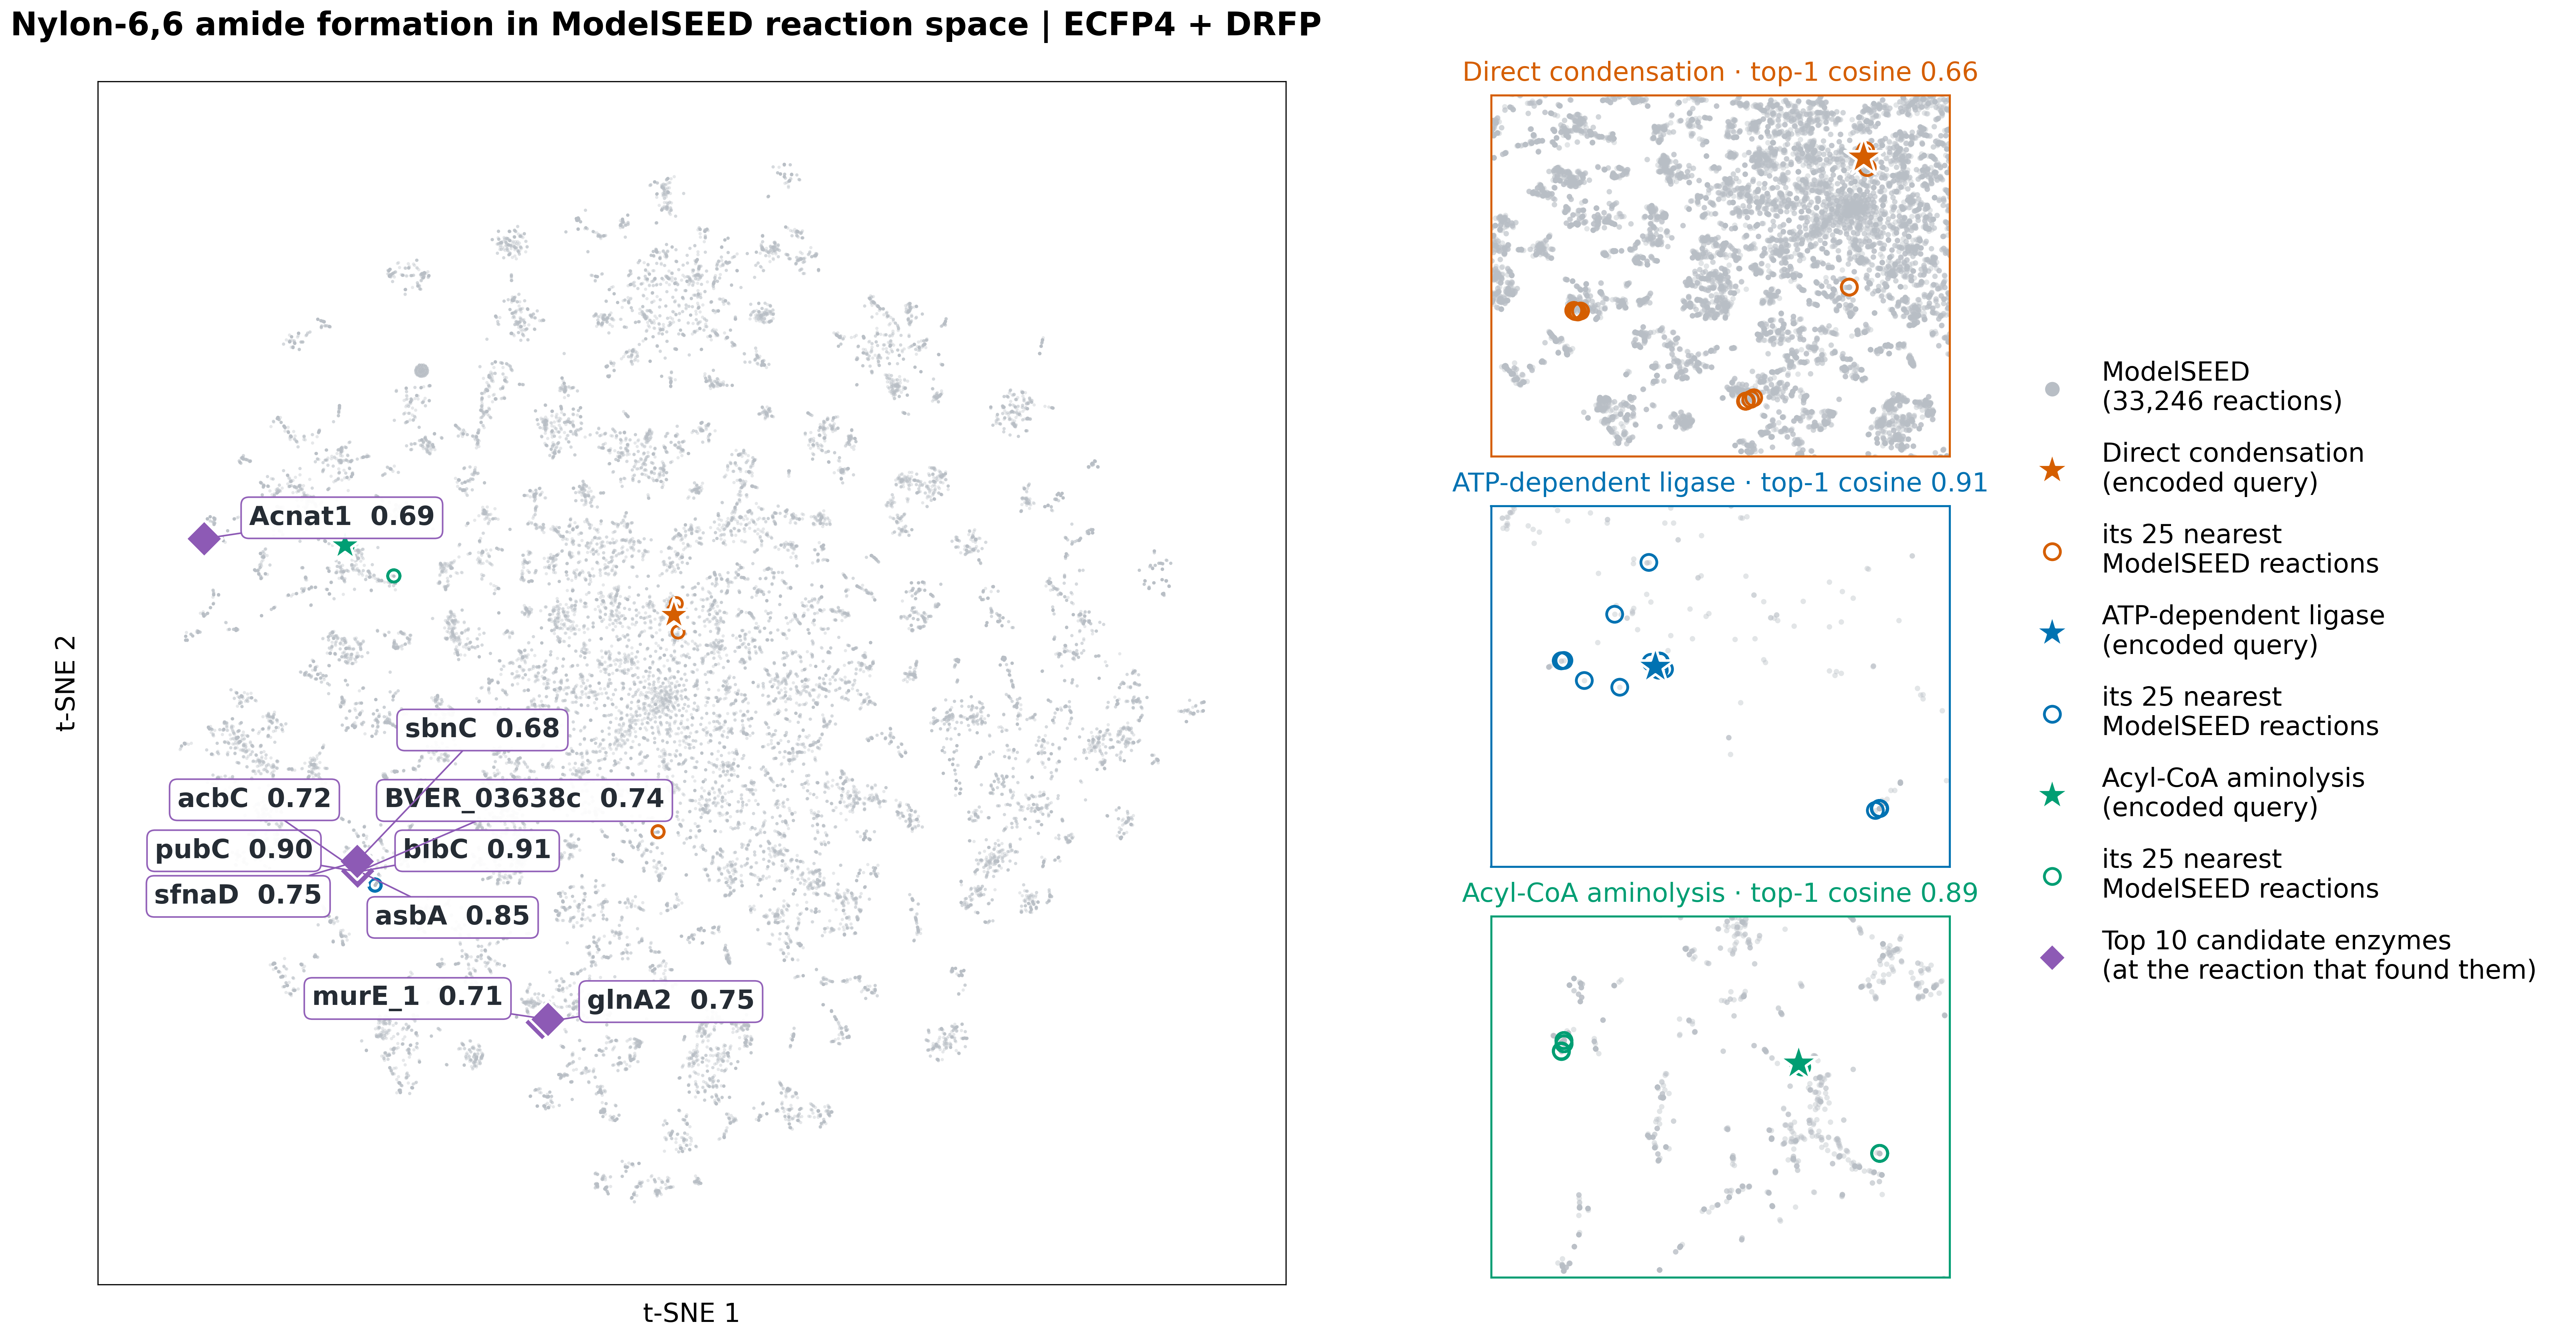
\includegraphics[width=0.93\linewidth,height=0.70\textheight,%
                   keepaspectratio]{fig_tsne_nylon_query.png}
  \takeaway{Diamonds are the top candidate enzymes, drawn at the reaction that
  retrieved them. t-SNE does not preserve cosine rank --- the ranking is
  authoritative, the map is for orientation.}
\end{frame}

% ---------------------------------------------------------------- caution
\begin{frame}{Cosine alone is not evidence of chemistry}
  A whole-reaction difference fingerprint is dominated by the largest
  compositional change --- \textbf{the cofactor}, not the amide bond.

  \medskip
  \begin{block}{Worked example}
    The acyl-CoA query's nearest EC-labelled neighbours are thioester
    \bad{hydrolases} (EC 3.1.2, agreement 0.80, no abstain). They make
    \textbf{no amide at all}; they merely release CoA.
  \end{block}

  \medskip
  Candidates therefore pass three \textbf{embedding-independent} screens,
  applied \emph{before} any top-$N$ cut:
  \begin{enumerate}
    \item a free amine is acylated --- proven by \textbf{cutting the product
      amide and reconstituting the parent amine}, which also \emph{names} the acceptor;
    \item that nitrogen is a genuine aliphatic amine (not aromatic, amide,
      nitrile or guanidino);
    \item the substrate is a small molecule, not a protein.
  \end{enumerate}

  \takeaway{33{,}246 reactions $\rightarrow$ \textbf{726} acylate a free amine
  $\rightarrow$ \textbf{482} eligible after excluding macromolecular (224, less
  5 polymer-elongation cases re-admitted) and unbalanced (22). \textbf{24
  curated screen controls} plus 327 unit tests guard this.}
\end{frame}

% ---------------------------------------------------------------- families
\begin{frame}{The hits converge on one family}
  \centering
  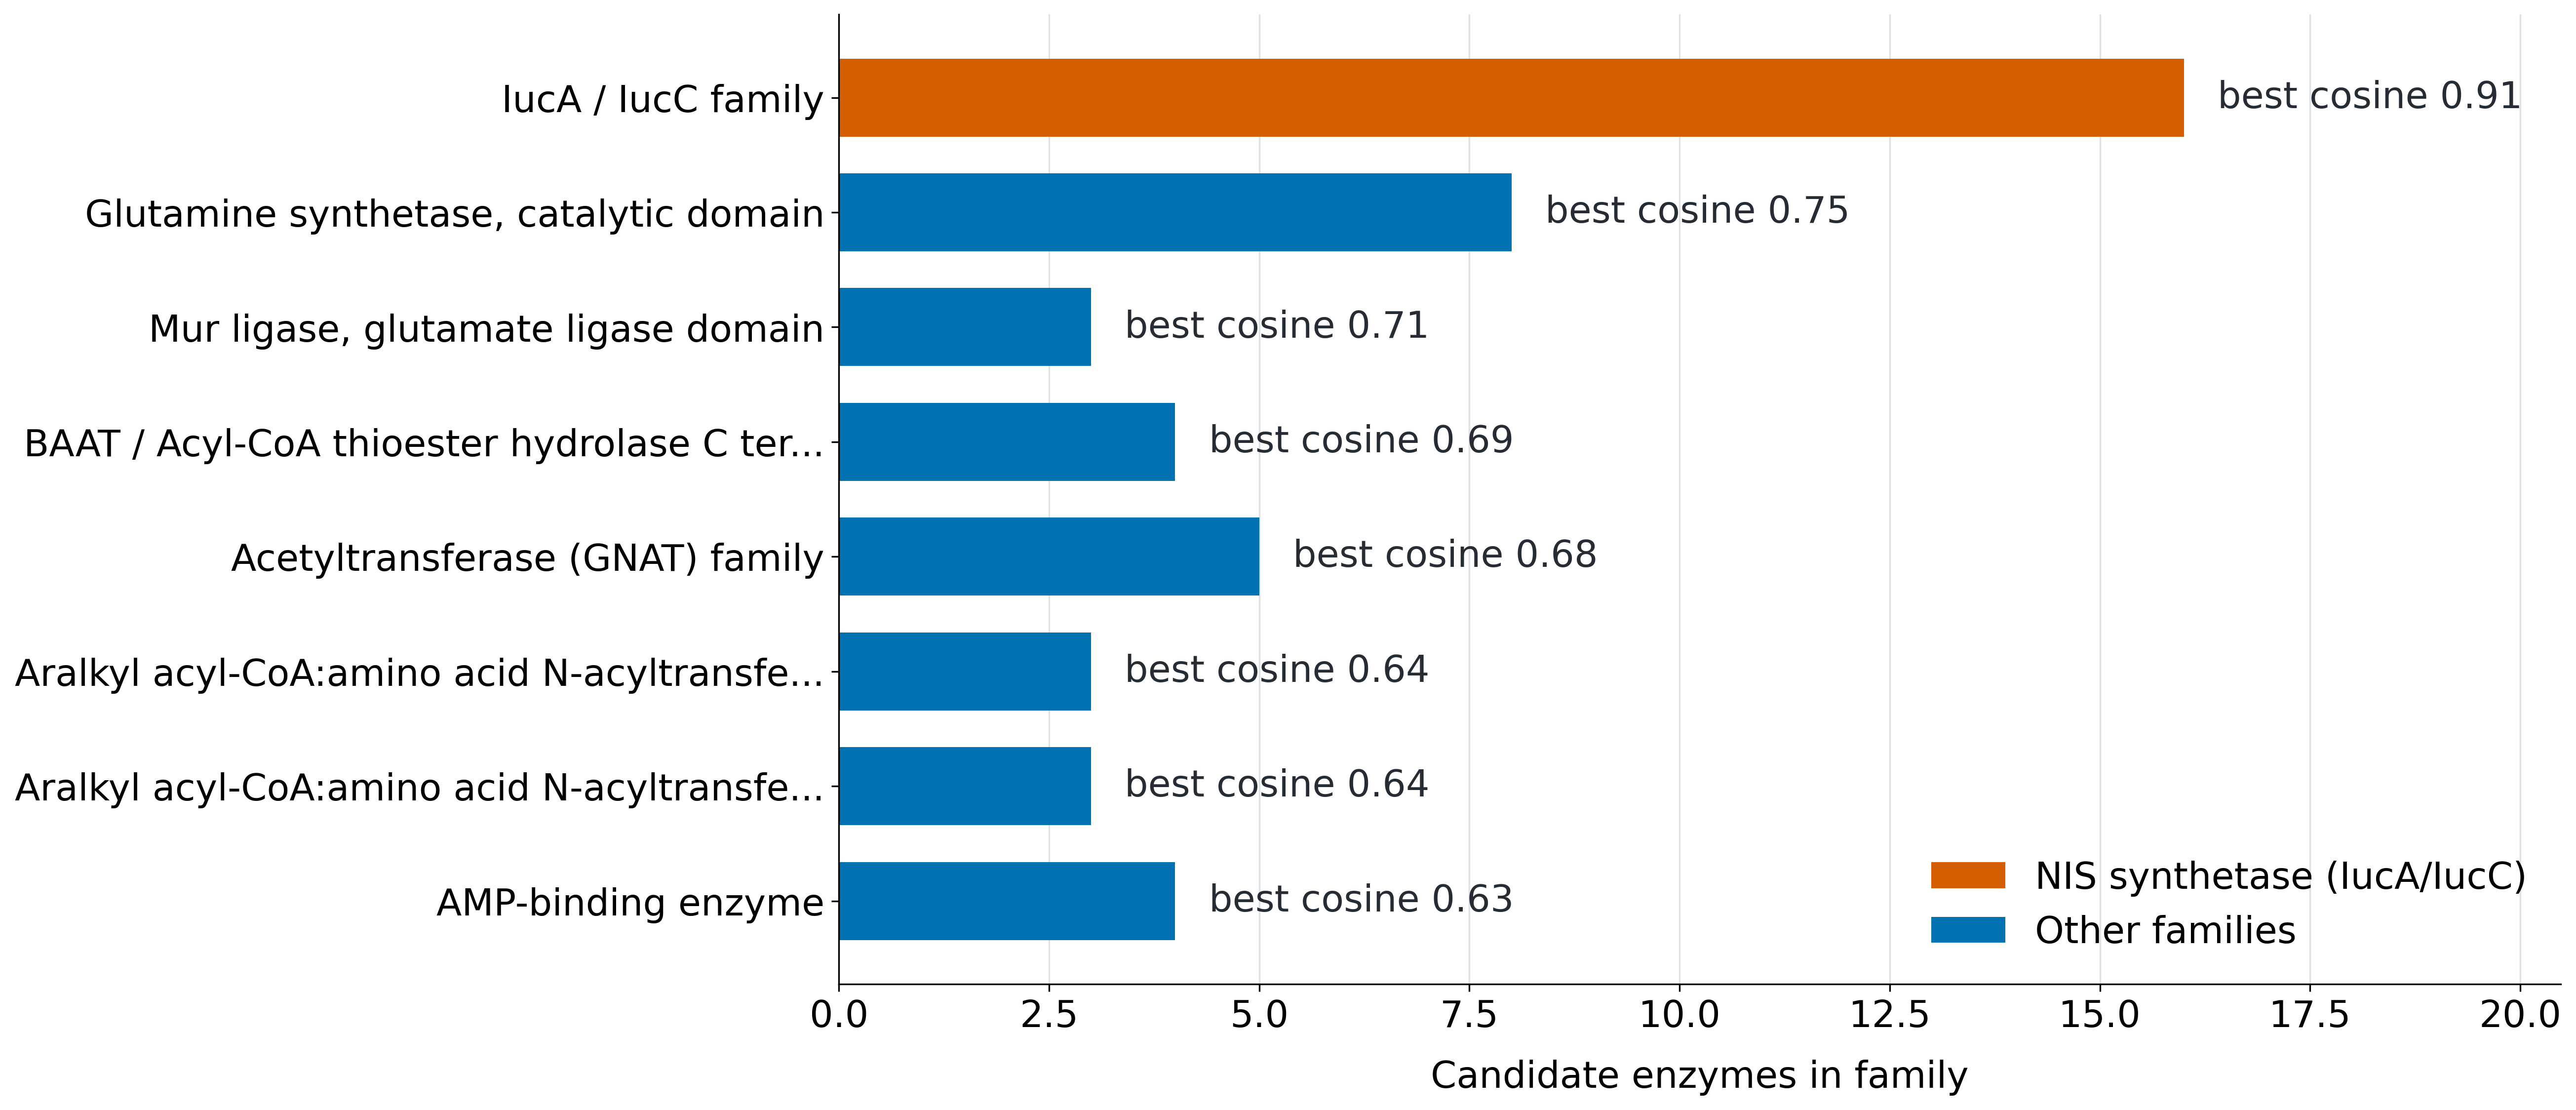
\includegraphics[width=0.82\linewidth]{fig_families.png}
  \takeaway{\nis{IucA/IucC --- the NIS (NRPS-independent siderophore)
  synthetases} --- is recovered 41 times over by independent seeds. One family
  found forty-one times is convergence, not forty-one independent hits.}
\end{frame}

% ---------------------------------------------------------------- chemistry
\begin{frame}{Why this family: they make polyamides}
  NIS synthetases form ATP-dependent amide bonds between carboxylic acids and
  \textbf{free polyamines} --- and several \textbf{iteratively oligomerise}
  bifunctional monomers into dimers and trimers.

  \medskip
  \centering
  \footnotesize
  \begin{tabular}{llrl}
    \toprule
    \textbf{Enzyme} & \textbf{Native reaction (UniProt, experimental)} & \textbf{Cosine} & \textbf{Family} \\
    \midrule
    \nis{BibC}  & 2 $\times$ succinyl-N-OH-cadaverine + 2 ATP $\rightarrow$ bisucaberin & \good{0.911} & \nis{IucA/IucC} \\
    \nis{PubC}  & 2 $\times$ succinyl-N-OH-putrescine + 2 ATP $\rightarrow$ putrebactin & \good{0.898} & \nis{IucA/IucC} \\
    AsbA        & spermidine + citrate + ATP $\rightarrow$ N$^8$-citryl-spermidine      & 0.851 & \nis{IucA/IucC} \\
    AsbB        & N$^8$-citryl-spermidine + spermidine + ATP (chain extension)          & 0.772 & \nis{IucA/IucC} \\
    SfnaD       & D-ornithine + citrate + ATP                                           & 0.753 & \nis{IucA/IucC} \\
    PuuA        & putrescine + L-glutamate + ATP $\rightarrow$ $\gamma$-Glu-putrescine  & 0.749 & Gln synthetase \\
    \bottomrule
  \end{tabular}

  \takeaway{BibC and PubC take \emph{one} bifunctional monomer and join it
  head-to-tail \textbf{twice}. That is polycondensation --- the same operation
  nylon-6,6 synthesis requires.}
\end{frame}

% ---------------------------------------------------------------- the key slide
\begin{frame}{The native substrate is the nylon diad's structural class}
  \centering
  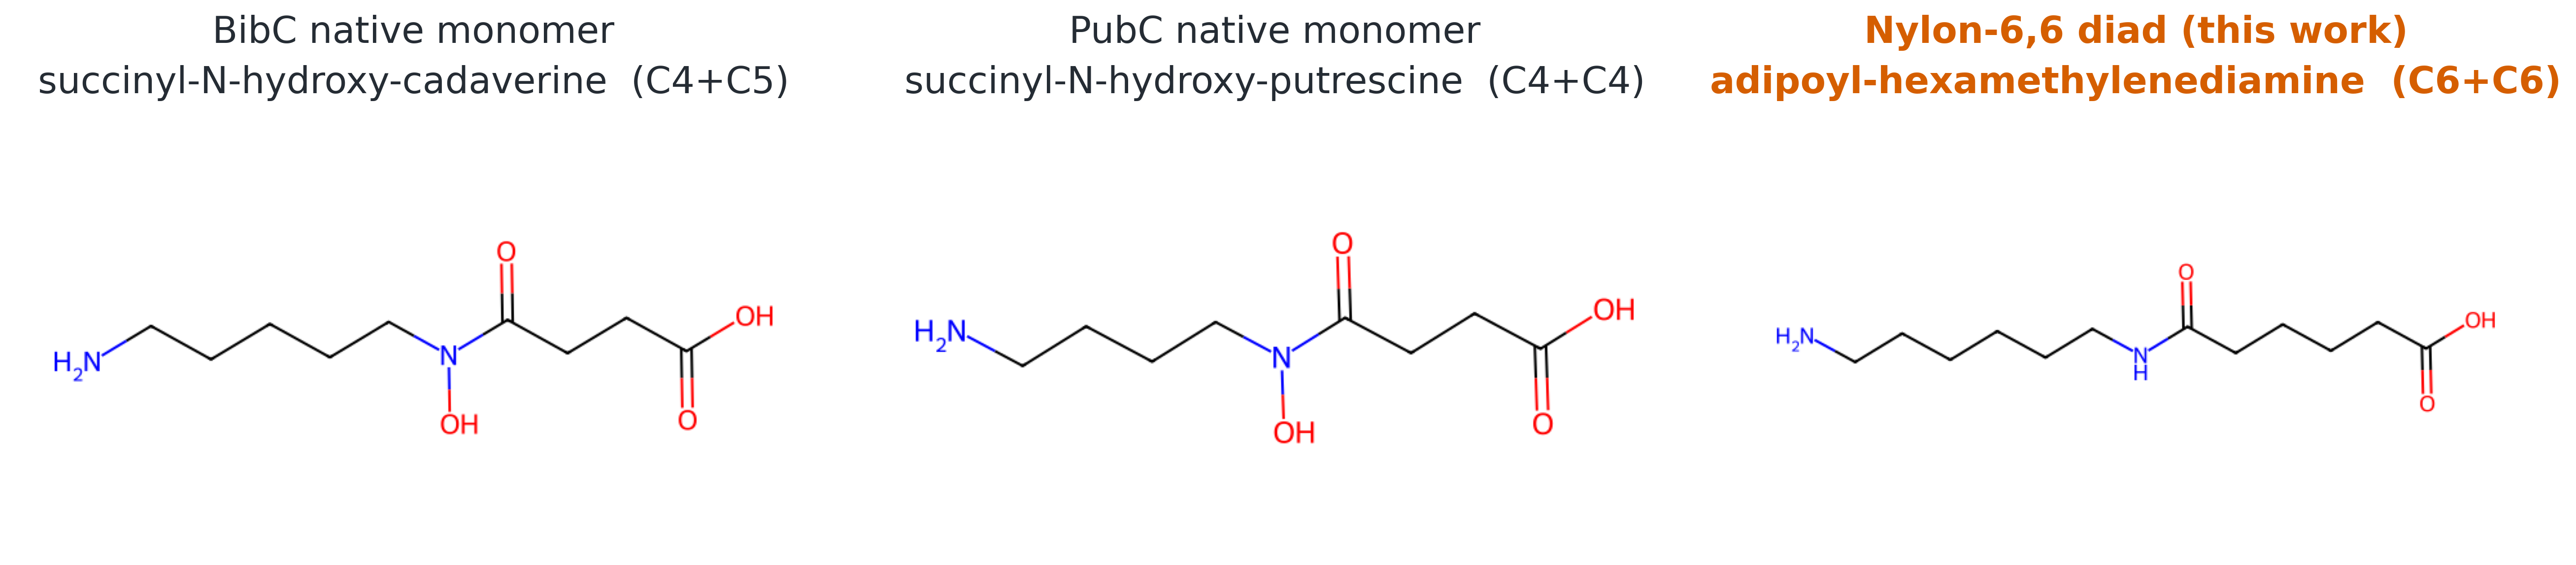
\includegraphics[width=\linewidth]{fig_substrate_gap.png}

  \medskip
  \begin{minipage}{0.92\linewidth}\small
    All three are \textbf{diamine--diacid half-amides}: free carboxylate at one
    end, free primary amine at the other. BibC and PubC natively \emph{dimerise}
    this exact motif.
  \end{minipage}

  \takeaway{This reframes the experiment: not only ``make the diad'', but
  \textbf{feed the pre-formed diad to BibC/PubC} and look for dimerisation ---
  the chain-extension step of nylon-6,6. \bad{Gap:} native monomers are
  N-hydroxylated and two carbons shorter per arm.}
\end{frame}

% ---------------------------------------------------------------- deliverable
\begin{frame}{Candidates for the bench}
  \centering
  \footnotesize
  \begin{tabular}{lllrl}
    \toprule
    \textbf{Enzyme} & \textbf{UniProt} & \textbf{Family} & \textbf{aa} & \textbf{Why test it} \\
    \midrule
    \nis{PubC}  & \texttt{P0DXD6}     & \nis{IucA/IucC} & 629 & cleanest dimerisation of a half-amide \\
    \nis{BibC}  & \texttt{B6EP94}     & \nis{IucA/IucC} & 819 & same, C5 monomer; highest cosine \\
    AsbA        & \texttt{A0A0F7RJ52} & \nis{IucA/IucC} & 602 & two \emph{different} monomers (AA/BB) \\
    AsbB        & \texttt{Q81RQ8}     & \nis{IucA/IucC} & 612 & chain extension; has a PDB structure \\
    PuuA        & \texttt{P78061}     & Gln synthetase  & 472 & \emph{E.~coli}; easiest expression/assay \\
    \bottomrule
  \end{tabular}

  \medskip
  \begin{block}{Deliverable}
    \texttt{results/shortlist\_annotated.tsv} --- a \textbf{301-protein}
    bench shortlist over \textbf{50 families} and 205 organisms, drawn from
    \textbf{54{,}199} candidates (2{,}048 Swiss-Prot reviewed). Carries
    \textbf{253 AlphaFold models} (median pLDDT \good{93.8}, none unusable),
    105 experimental structures, 41 cofactor-bound, \textbf{194 proteins with
    a measured $K_M$/$k_{cat}$}, and 48 with \textbf{measured nylon-6,6 titre}.
  \end{block}

  \takeaway{Similarity is to \emph{reactions}. No listed enzyme is known to
  accept adipate or HMDA --- this analysis \textbf{generates} that hypothesis,
  it does not validate it.}
\end{frame}

% ---------------------------------------------------------------- routes
\begin{frame}{ModelSEED has no reaction $\rightarrow$ enzyme mapping}
  So breadth comes from having \textbf{seven independent bridges}, not one good
  one. Every row records which produced it.

  \smallskip
  \centering\footnotesize
  \begin{tabular}{llr}
    \toprule
    \textbf{Route} & \textbf{What it claims} & \textbf{Candidates} \\
    \midrule
    \texttt{reaction}          & annotated to a screened ModelSEED reaction & 816 \\
    \texttt{precomputed\_link} & a global UniProt$\rightarrow$ModelSEED table & 2{,}554 \\
    \texttt{domain}            & Pfam/InterPro family with \emph{characteristic} chemistry & 9{,}365 \\
    \texttt{clade}             & UniRef50 neighbourhood of a validated protein & 36{,}889 \\
    \texttt{enzyme\_name}      & UniProt \emph{names} it for the target function & 4{,}512 \\
    \texttt{assayed}           & \good{measured nylon-6,6 titre} & 49 \\
    \texttt{proxied}           & literature-curated, carries a geometric score & 14 \\
    \bottomrule
  \end{tabular}

  \takeaway{\textbf{ModelSEED is not the bottleneck.} Screening all 36{,}552
  Rhea reactions with our own screen found \textbf{417} amide-forming reactions
  unreachable from ModelSEED --- and they yield \bad{3} proteins, because 21 of
  the top 25 have \emph{no enzyme annotated at all}. The missing links do not
  exist.}
\end{frame}

% ---------------------------------------------------------------- gates
\begin{frame}{A score must rank retrieval, never gate it}
  Cosine on a whole-reaction fingerprint is dominated by the cofactor, yet it
  was deciding \emph{which reactions were ever looked at} --- in five places,
  including one this project added itself.

  \smallskip
  \centering\footnotesize
  \begin{tabular}{llr}
    \toprule
    \textbf{Gate} & \textbf{What it discarded} & \textbf{Cost} \\
    \midrule
    \texttt{TOPN=30} per query      & 41 of the 62 best-scoring reactions & \bad{high} \\
    \texttt{priority} tie-break     & broke every tie on cosine & now \good{zero} \\
    OOD floor on admission          & 96 of 205 reactions, the \emph{highest}-scoring & all FPGS, all Mur \\
    stage 04 re-litigating stage 03 & \texttt{rxn14123} at cosine 0.499 vs floor 0.5041 & 126 proteins \\
    \bad{our own} \texttt{SD\_FLOOR=0.40} & 214 of 482 \emph{screen-proven} reactions & see below \\
    \bottomrule
  \end{tabular}

  \takeaway{Removing our own floor: reactions resolved 168 $\rightarrow$
  \good{308}, candidates $+2{,}021$ --- and annotation coverage went \emph{up}.
  Gating on a score discards evidence; ranking on it does not.}
\end{frame}

% ---------------------------------------------------------------- families
\begin{frame}{Judge the family, not just the protein}
  A protein admitted by family membership \textbf{inherits} its family's score,
  so the decision governing tens of thousands of candidates is made once per
  family. It is now made explicitly, on the \emph{measured} chemistry of each
  family's own validated seeds.

  \smallskip
  \centering
  \begin{tabular}{lrl}
    \toprule
    \textbf{Verdict} & \textbf{n} & \textbf{Criterion} \\
    \midrule
    \good{lead}  & 54 & diacid + diamine, self-condensing, or bifunctional one side \\
    watch        & 16 & monofunctional, or the donor drags a large scaffold \\
    \bad{reject} & 33 & terminal amide, or the members contradict the chemistry \\
    \bottomrule
  \end{tabular}

  \smallskip
  \begin{block}{What seed chemistry alone misses}
    $\gamma$-glutamyltranspeptidase scores 0.64 on its seeds and looked like a
    lead --- while \bad{1{,}550 of its 1{,}594 members} are annotated as a
    non-amide-forming activity. It is a hydrolase family running a
    transpeptidation side reaction.
  \end{block}

  \takeaway{103 families from 298 Pfam/InterPro signatures; the verdict
  \textbf{prunes 8{,}409} candidates from the bench list. This is the lever
  that makes the search more \emph{targeted}, not larger.}
\end{frame}

% ---------------------------------------------------------------- caveats
\begin{frame}{What we found along the way}
  \begin{block}{The 2026-10-06 ModelSEED structure refresh is wrong for amides}
    $\sim$17\% of compounds --- including NAD, NADH, NADP, CoA, every acyl-CoA,
    nicotinamide --- write carboxamides as \bad{iminols} (\texttt{C([O-])=N} and
    \texttt{C(O)=N}), with adenine N1 as \texttt{[nH+]}. An iminol is
    \textbf{invisible to an amide SMARTS}. 6{,}313 compounds repaired; the repair
    reproduces the previous snapshot exactly.
  \end{block}

  \begin{block}{Honest limitations}
    \begin{itemize}
      \item The repair is \emph{not} charge-neutral (5{,}807 compounds shift
        charge), so the corpus audits balance separately; unbalanced reactions
        are excluded, not hidden.
      \item BibC and PubC carry \textbf{no Rhea and no EC in ModelSEED}; both
        were recovered by pivoting through \textbf{MetaNetX}. 308 of 482
        screened reactions resolve to an enzyme.
      \item Screens are structural inference, not atom-mapped proof.
    \end{itemize}
  \end{block}

  \takeaway{Reproducible by \texttt{run\_all.py}: 23 stages, $\sim$40 min,
  mostly polite API querying; 327 unit tests, 24 screen controls.}
\end{frame}

\end{document}
